\section{Introduction}
Hierarchical clustering is a way to recursively partition a dataset into clusters. The data is usually represented by a weighted, connected graph $G = (V, E, c)$, where $c\colon E\to \mathbb{N}$ is the \emph{similarity} measure between the points. The goal is to find a rooted tree called \textit{clustering tree} $T$, in which every node $u\in V\br{T}$ represents a connected component $G_u\subseteq G$ called a \textit{cluster}. Moreover, every non-leaf node $u$ of $T$ corresponds to a subset of edges $S_u$ such that for every child node $v$ of $u$, $G_v\in G_u\setminus S_u$. For each leaf node $l\in V\br{T}$ it is required that $G_l$ is a singleton, i.~e., $\spr{V\br{G_l}}=1$. Then, the \textit{Dasgupta's clustering objective} is defined as $\COST_G\br{T} = \sum_{u\in V\br{T}} c(S_u) \cdot |V(G_u)|$\footnote{Note that the usual way of defining the Dasgupta's clustering objective is $\COST_G\br{T} = \sum_{uv\in E} c(uv) \cdot |\ell_T\br{u,v}|$, where $\ell_T\br{u,v}$ denotes the smallest subtree containing both $u$ and $v$. It is easy to see, that our formulation is equivalent and we use it for the sake of convenience.}. The problem of finding a clustering tree which minimizes the above cost is known as the \textsc{Hierarchical Clustering} problem and is NP-hard~\cite{ACostFunctionForSimilarityBasedHierarchicalClustering}. Intuitively, the Dasgupta's clustering objective `punishes' cutting edges with high similarity early on in the clustering tree, since the larger the component in which the edge is cut, the higher the contribution of this edge to the cost.

The main advantage of the hierarchical clustering over various kinds of flat clustering is that it provides a decomposition of the data which is not reliant on the granularity of subdivision one wishes to acquire. Since the clusters are refined until they become singletons, the hierarchy encodes various granularity levels into it. However, it is often implicitly assumed that eventually all of them need to become singletons. In this work we ask the following question: What would happen if we relax the halting condition of the recursive partitioning process and allow it to stop whenever the remaining cluster is a graph of some class $\cF$? 
We will assume, that the graph class $\cF$ is a part of the input and represents some kind of structural property which is deemed `simple' enough so that there is no need to further refine the clusters\footnote{Here, we assume that $\cF$ is non-empty and closed under taking subgraphs, which ensures that any subcluster of a cluster in $\cF$ also belongs to $\cF$. Moreover, for the sake of practicality it is reasonable to assume that the class $\cF$ is recognizable in polynomial time. Otherwise, the task of constructing any clustering tree at all becomes intractable and the pursuit of approximation algorithms becomes futile as well.}.
Therefore we only require that for each leaf node $l\in V\br{T}$, $G_l\in \cF$. We call this problem \textsc{Hierarchical $\cF$-Clustering} (HC-$\cF$). The goal is again to minimize $\COST_G\br{T} = \sum_{u\in V\br{T}} c(S_u) \cdot |V(G_u)|$. For a visual example of a clustering tree for \textsc{HC-$\cT$}, where $\cT$ denotes the class of trees see Figure~\ref{fig:hac-intro-example}.
\DDfix{
We note that the objective value for HC-$\cF$ may be quite different from that of the classical hierarchical clustering.
If the input graph $G$ belongs to $\cF$, then $\COST_G\br{T}=0$ for a single-node $T$ with root representing $G$.
On the other hand, one may have, even for unit costs, $\COST_G\br{T}=\Omega\br{n^2}$ for $T$ whose leaves are singletons.
}
\begin{figure}[H]
    \centering
    \begin{minipage}[t]{0.46\textwidth}
        \centering
        \begin{tikzpicture}[scale=0.95, every node/.style={circle,draw,fill=white,inner sep=1.5pt,font=\scriptsize,preaction={fill=black,opacity=0.18,transform canvas={xshift=0.8pt,yshift=-0.8pt}}}]
            \node (a1) at (-2.6,1.8) {$a$};
            \node (a2) at (-3.6,0.8) {$b$};
            \node (a3) at (-3.0,-0.6) {$c$};
            \node (a4) at (-1.8,-0.6) {$d$};
            \draw[cutB,very thick] (a1)--(a2);
            \draw (a2)--(a3);
            \draw (a3)--(a4);
            \draw[cutB,very thick] (a4)--(a1);
            \draw (a1)--(a3);

            \node (b1) at (-0.2,1.4) {$e$};
            \node (b2) at (0.7,0.9) {$f$};
            \node (b3) at (0.3,-1.1) {$g$};
            \node (b4) at (-1.0,0.0) {$h$};
            \draw[cutD,very thick] (b1)--(b2);
            \draw (b2)--(b3);
            \draw (b3)--(b4);
            \draw (b4)--(b1);

            \node (c1) at (2.8,1.8) {$i$};
            \node (c2) at (3.8,0.8) {$j$};
            \node (c3) at (3.2,-0.6) {$k$};
            \node (c4) at (2.0,-0.6) {$l$};
            \draw[cutE,very thick] (c1)--(c2);
            \draw[cutF,very thick] (c2)--(c3);
            \draw (c3)--(c4);
            \draw[cutE,very thick] (c4)--(c1);
            \draw (c2)--(c4);

            \node (x1) at (-1.5,1.1) {$m$};
            \node (x2) at (1.95,1.95) {$n$};
            \draw[cutB,very thick] (x1)--(a1);
            \draw (x1)--(a4);
            \draw[cutA,very thick] (x1)--(b1);
            \draw[cutC,very thick] (x2)--(b2);
            \draw[cutC,very thick] (x2)--(b3);
            \draw (x2)--(c1);
            \draw[cutE,very thick] (x2)--(c4);
            \draw[cutA,very thick] (a4)--(b4);
            \draw[cutC,very thick] (b4)--(c4);
        \end{tikzpicture}
        \\\smallskip
        {\small An input graph $G$ with 14 vertices.
        For all edges $e$, we have $c(e)=1$.}
    \end{minipage}
    \begin{minipage}[t]{0.52\textwidth}
        \centering
        \begin{tikzpicture}[x=0.85cm,y=0.72cm, hcnode/.style={draw,rounded corners,fill=white,inner sep=2pt,font=\scriptsize,align=center,preaction={fill=black,opacity=0.18,transform canvas={xshift=0.8pt,yshift=-0.8pt}}}]
            \node[hcnode] (r) at (0,0) {$V(G)$\\cut: $\{\textcolor{cutA}{em},\textcolor{cutA}{dh}\}$};
            \node[hcnode,anchor=north] (u1) at ([xshift=-1.60cm,yshift=-0.09cm]r.south) {$\{a,b,c,d,m\}$\\cut: $\{\textcolor{cutB}{ab},\textcolor{cutB}{ad},\textcolor{cutB}{am}\}$};
            \node[hcnode,anchor=north] (u2) at ([xshift=1.60cm,yshift=-0.09cm]r.south) {$\{e,f,g,h,i,j,k,l,n\}$\\cut: $\{\textcolor{cutC}{fn},\textcolor{cutC}{gn},\textcolor{cutC}{lh}\}$};
            \node[hcnode,anchor=north] (v1) at ([xshift=-0.80cm,yshift=-0.11cm]u1.south) {$\{a,b,c,d,m\}$};
            \node[hcnode,anchor=north] (w1) at ([xshift=-1.10cm,yshift=-0.11cm]u2.south) {$\{e,f,g,h\}$\\cut: $\{\textcolor{cutD}{ef}\}$};
            \node[hcnode,anchor=north] (w2) at ([xshift=1.10cm,yshift=-0.11cm]u2.south) {$\{i,j,k,l,n\}$\\cut: $\{\textcolor{cutE}{nl},\textcolor{cutE}{li},\textcolor{cutE}{ij}\}$};
            \node[hcnode,anchor=north] (z1) at ([xshift=-0.40cm,yshift=-0.11cm]w1.south) {$\{e,f,g,h\}$};
            \node[hcnode,anchor=north] (z2) at ([xshift=-1.10cm,yshift=-0.11cm]w2.south) {$\{i,n\}$};
            \node[hcnode,anchor=north] (z3) at ([xshift=1.10cm,yshift=-0.11cm]w2.south) {$\{j,k,l\}$\\cut: $\{\textcolor{cutF}{kj}\}$};
            \node[hcnode,anchor=north] (t1) at ([xshift=0.00cm,yshift=-0.11cm]z3.south) {$\{j,k,l\}$};

            \node[draw=none,fill=none,preaction={},anchor=west,xshift=0.09cm,font=\tiny,align=center] at (r.east) {cost:\\$2\cdot 14$};
            \node[draw=none,fill=none,preaction={},anchor=east,xshift=-0.09cm,font=\tiny,align=center] at (u1.west) {cost:\\$3\cdot 5$};
            \node[draw=none,fill=none,preaction={},anchor=west,xshift=0.09cm,font=\tiny,align=center] at (u2.east) {cost:\\$3\cdot 9$};
            \node[draw=none,fill=none,preaction={},anchor=east,xshift=-0.09cm,font=\tiny,align=center] at (w1.west) {cost:\\$1\cdot 4$};
            \node[draw=none,fill=none,preaction={},anchor=west,xshift=0.09cm,font=\tiny,align=center] at (w2.east) {cost:\\$3\cdot 5$};
            \node[draw=none,fill=none,preaction={},anchor=west,xshift=0.09cm,font=\tiny,align=center] at (z3.east) {cost:\\$1\cdot 3$};

            \draw (r)--(u1);
            \draw (r)--(u2);
            \draw (u1)--(v1);
            \draw (u2)--(w1);
            \draw (u2)--(w2);
            \draw (w1)--(z1);
            \draw (w2)--(z2);
            \draw (w2)--(z3);
            \draw (z3)--(t1);
        \end{tikzpicture}
        \\\smallskip
        {\small A hierarchical clustering tree $T$ of cost $2\cdot14+3\cdot5+3\cdot9+1\cdot4+3\cdot5+1\cdot3=92$.}
    \end{minipage}
    \caption{Example of an instance of \textsc{HC-$\cT$} and a feasible hierarchical clustering: Colors denote edges cut at different levels of the tree.}
    \label{fig:hac-intro-example}
\end{figure}


\subsection{Motivations and applications}
Hierarchical clustering is a clustering technique that is far richer in structure and applications than traditional flat clustering. Since such an object encodes a hierarchical decomposition of data, one may choose an appropriate granularity level of clustering according to their needs. 
Phylogenetic trees, file systems, company management hierarchies, and socio-political divisions are all examples of hierarchical clusterings. Relaxing the halting condition of the clustering process has intuitive applications both for the case of trees as well as bounded-diameter graphs. It is easy to see, that not all of the aforementioned hierarchies finish on singleton objects. For example file systems often contain directories with multiple files. To seek more such examples, one may consider a categorization of products available in a given online store, where one bottom category may contain a very large amount of objects. It seems desirable to find a way to systematically build such structures, especially since a well-structured e-commerce platform is crucial for the success of the business. Here, it would be required for the bottom clusters to consists of products which are similar enough to be considered as a single category.
Enforcing bounded-diameter clusters is therefore a natural requirement, since such clusters aggregate points that are close to one another. Note, that in our setting, the cost function encodes similarity between objects, which inflates the diameter of the clusters when the similarity is higher. Luckily, it turns out that our diameter restrictions can be defined with respect to any metric, not limited to the similarity function or the number of edges.
% Trees are among simplest classes of graphs and therefore most of their structural properties are well understood. Additionally, many problems which are hard on general graphs can be solved efficiently on trees.  

Among possible usages of clustering into trees is the following heuristic for the standard \textsc{HC}. Firstly, run an algorithm for \textsc{HC-$\cT$} to obtain a clustering tree $T$ such that for each leaf $l$ of $T$, $G_l$ is a tree. Next, for each such $G_l$, run any algorithm for \textsc{HC} on trees to recover the remaining levels of clusterization. Since \textsc{HC} on trees admits a polynomial-time constant-factor approximation~\cite{ApproximateHierarchicalClusteringViaSparsestCutAndSpreadingMetrics}, the dominant part of the total approximation error comes from computing the solution for \textsc{HC-$\cT$}. Consequently, the better the approximation algorithm for \textsc{HC-$\cT$}, the better the performance of this heuristic.
The resulting clustering tree can also be used partially dynamically: the $\cT$-clustering tree may be stored statically, and whenever a leaf cluster needs refinement, we can run an \textsc{HC} algorithm on that leaf. In this way, we obtain a partially dynamic clustering tree which occupies less space than a full \textsc{HC} tree, while still allowing on-demand refinement.


% \begin{figure}[H]
    \centering
    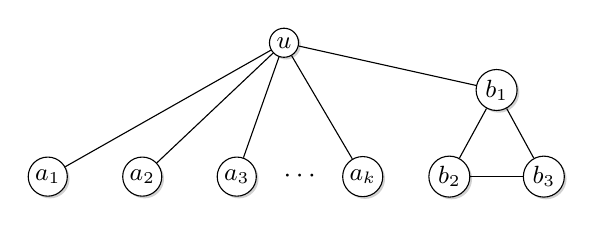
\begin{tikzpicture}[vtx/.style={circle,draw,fill=white,inner sep=1.4pt,font=\small,preaction={fill=black,opacity=0.18,transform canvas={xshift=0.8pt,yshift=-0.8pt}}}]
        \node[vtx] (u) at (0.8,0) {$u$};
        \node[vtx] (a1) at (-2.2,-1.7) {$a_1$};
        \node[vtx] (a2) at (-1.0,-1.7) {$a_2$};
        \node[vtx] (a3) at (0.2,-1.7) {$a_3$};
        \node[vtx] (ak) at (1.8,-1.7) {$a_k$};
        \node (dots) [draw=none,fill=none,preaction={},shape=rectangle,inner sep=0pt,outer sep=0pt,minimum size=0pt] at (1.0,-1.7) {$\cdots$};

        \node[vtx] (b1) at (3.5,-0.6) {$b_1$};
        \node[vtx] (b2) at (2.9,-1.7) {$b_2$};
        \node[vtx] (b3) at (4.1,-1.7) {$b_3$};

        \draw (u) -- (a1);
        \draw (u) -- (a2);
        \draw (u) -- (a3);
        \draw (u) -- (ak);
        \draw (u) -- (b1);

        \draw (b1) -- (b2);
        \draw (b2) -- (b3);
        \draw (b3) -- (b1);
    \end{tikzpicture}
    \caption{Example of graph for which the multiplicative difference between values of both clustering objective functions is $\Theta\br{n}$.}
    \label{fig:star-triangle-example}
\end{figure}

%
% We also remark that despite their similarity, the objective value of \textsc{HC-$\cF$} can be much smaller than that of \textsc{HC}. Consider $\cF=\cT$. Let $G$ be a star in which one vertex is replaced by a triangle, and assume uniform edge costs. The optimal clustering tree for \textsc{HC} has cost $\Omega\br{n^2}$, since at least $(n-2)/2$ vertices must have at least $(n-2)/2$ edges cut before becoming singletons. In contrast, the optimal clustering tree for \textsc{HC-$\cT$} has cost $n$, since the optimum consists of cutting a single edge of the triangle. This example shows that the structure of the optimum clustering tree for \textsc{HC-$\cT$} can differ significantly from \textsc{HC}. A similar example for $_d$-clusters is obtained by picking $d=1$ and letting the input graph be a clique. Here, the optimal clustering tree for \textsc{HC} has cost $\Omega\br{n^2}$, while the optimal clustering tree for \textsc{HC-$\cD_1$} has cost $0$, since the whole graph is a valid cluster.

\subsection{Our results and techniques}

Our main contribution is a general framework for approximating \textsc{HC-$\cF$} problems for classes of graphs $\cF$, which we call $\alpha\br{n}$-well-behaved. This means, that there exists a natural, cover-like ILP formulation of the \textsc{$p_{\cF}$-Partitioning} (\textsc{$p_{\cF}$-P}) problem (see Problem~\ref{prob:pfp}) as well as an algorithm which given a solution to the LP relaxation of this ILP, finds a solution to \textsc{$p_{\cF}$-P} with cost at most $\alpha\br{n}$ times the cost of the LP solution. This results in an $O\br{\alpha\br{n}+\beta\br{n}}$-approximation algorithm for \textsc{HC-$\cF$}, where $\beta\br{n}$ is the approximation ratio of the LP-based bicriteria algorithm for \textsc{$\rho$-SEP} (Problem~\ref{prob:rho-sep}), currently at $\beta\br{n}=O\br{\log n}$. As an immediate corollary we obtain an $O\br{\log n\cdot\log\log n}$-approximation algorithm for clustering into trees and an $O\br{\log n}$-approximation algorithm for clustering into clusters of diameter at most $d$. To the best of our knowledge, these are the first algorithmic results for the \textsc{HC-$\cF$} problem.

Conceptually, our work follows an implicitly, but broadly used technique which hereby we call \textit{flattening}. The idea is to subdivide the problem of finding a hierarchical/temporal\footnote{It is worth mentioning, that the hierarchical clustering tree can be treated as a sort of schedule of edges to be cut. This interpretation suggest that the depth of the tree can be treated as the time dimension of that schedule.} object such as a clustering tree into a problem of finding a sequence of `flat' objects such as separators or cuts. Among multiple uses of such a technique, one can mention \textsc{Hierarchical Clustering}~\cite{ACostFunctionForSimilarityBasedHierarchicalClustering, ApproximateHierarchicalClusteringViaSparsestCutAndSpreadingMetrics,Hierarchical_Clustering_Objective_Functions_and_Algorithms}, \textsc{Graph Search Problem}~\cite{Approximating_the_Average_Case_Graph_Search_Problem_with_Non_uniform_Costs}, \textsc{Tree Decompositions}~\cite{Approximating_Treewidth_Pathwidth_Frontsize_and_Shortest_Elimination_Tree}, \textsc{Precedence-Constrained Decision Tree}~\cite{Precedence-Constrained_Decision_Trees_and_Coverings} and many more.

Our ideas are particularly inspired by the work of Charikar and Chatziafratis~\cite{ApproximateHierarchicalClusteringViaSparsestCutAndSpreadingMetrics}, who used the flattening technique in conjunction with the \emph{spreading-metrics} framework. Whereas they used SDP relaxation, we encode the structure of the clustering tree using linear programming. The LP is divided into levels which allow decomposing it into several, level-restricted guides, which serve as a blueprint for the recursive construction of the clustering tree.
As it turns out, in order to encode the structural requirements given by the class $\cF$, we refine their technique by enriching the ILP formulation of the problem with generalized type of constraints which encode whether the clusters at each level have the desired properties. This is due to the fact that we need to force the ILP to optimize for two types of measures of progress: cutting edges required to transform clusters into $\cF$-clusters as well as efficient graph partitioning. Since $\cF$ might be an (almost) arbitrary class of graphs, we aim at showcasing a general framework of solving such problems, rather then focusing on singular solutions. To achieve this, we enforce certain natural conditions on the input family $\cF$, which in particular are satisfied by the graph classes of our interest. Any graph class respecting those conditions is called \emph{$\alpha\br{n}$-well-behaved}. Of particular importance is to us the notion of $\cF$-predicate which is a boolean function encoding whether a given vertex satisfies some structural property such that if all vertices of a graph satisfy the $\cF$-predicate, then all of the clusters are guaranteed to belong to $\cF$. Such a property can be for example whether a given vertex belongs to a cycle. If a given $\cF$ respects these conditions, we automatically get a series of constraints which will get included into our ILP, and this will suffice for a good approximation guarantee.

In order to extract useful information out of our ILP, we relax it into an LP and solve it (in polynomial time). Upon doing so, we use a simple arithmetic rounding procedure to fix the values of the $\cF$-predicate. Since our LP is organized into levels mimicking the levels of the hierarchy, we \DDfix{(recursively)} decompose the solution according to those level and then use an LP-guided recursive processing in order to find the clustering tree.
At each recursion step, the algorithm uses the fragment of the LP on the current level to find two sets of edges to cut. The first, such that for each vertex $v$ in the current cluster, for which the LP value of the $\cF$-predicate is 1, the $\cF$-predicate is satisfied. The second, such that the remaining clusters are small enough. The algorithm then builds the rest of the clustering tree recursively. Using a careful lower bounding of the cost we get that the approximation ratio of our algorithm is $O\br{\alpha\br{n}+\beta\br{n}}$.

To complement the algorithmic results, we show that for both $\cT$ and $\cD_d$ the problem cannot be approximated within any constant factor under the Small Set Expansion Hypothesis~\cite{GraphExpansionAndTheUniqueGamesConjecture}. We use a blackbox reduction from the inapproximability of \textsc{Hierarchical Clustering}~\cite{ApproximateHierarchicalClusteringViaSparsestCutAndSpreadingMetrics} by adding appropriate gadgets to all of the vertices of the original graph. Importantly, for the case of $\cF=\cT$ we use a structural property observed by the authors above, that the cost of the optimal solution to \textsc{HC} is lower bounded by the cost of the \textsc{Minimum Linear Arrangement}. Notably, this may no longer be true for the case for an arbitrary instance of \textsc{HC-$\cT$}, but we show that a similar lower bound still holds true for our construction.
\subsection{Related Work}

\paragraph{Flat Clustering}
Classical flat clustering objectives include \textsc{$k$-Center}, \textsc{$k$-Median}, and \textsc{$k$-Means}. For metric \textsc{$k$-Center}, a simple greedy farthest-first traversal yields a $2$-approximation, and this factor is optimal unless $P=NP$~\cite{GonzalezKCenter, HochbaumShmoysKCenter}. For metric \textsc{$k$-Median}, many constant factor approximation algorithms are known~\cite{AConstant-FactorApproximationAlgorithmForTheKMedianProblem, ApproximationAlgorithmsForMetricFacilityLocationAndKMedianProblemsUsingThePrimal-DualSchemaAndLagrangianRelaxation, ANewGreedyApproachForFacilityLocationProblems, AryaLocalSearchKMedian, Approximating_k-Median_via_Pseudo-Approximation, AnImprovedApproximationForKMedianAndPositiveCorrelationInBudgetedOptimization,BreachingThe2LMPApproximationBarrierForFacilityLocationWithApplicationsToKMedian} culminating in $\br{2+\epsilon}$ approximation of~\cite{A2-ApproximationAlgorithmForMetricKMedian}. For metric \textsc{$k$-Means}, constant-factor approximations are also known (for example via local search), with improved guarantees in Euclidean settings~\cite{KanungoKMeansLocalSearch, AhmadianKMeansImprovedApprox} with the currently best known guarantee of $3+2\sqrt{2}+\epsilon< 5.83$~\cite{AnImprovedGreedyApproximationForMetricKMeans}.

\paragraph{\textsc{Hierarchical Clustering}}
Work on \textsc{Hierarchical Clustering} can be split into similarity-based and dissimilarity-based objectives. In the similarity-based setting, Dasgupta introduced the now standard objective and initiated its approximation-theoretic study~\cite{ACostFunctionForSimilarityBasedHierarchicalClustering}. This line was further developed by Charikar and Chatziafratis, who obtained an $O(\sqrt{\log n})$-approximation via \textsc{Sparsest Cut} and spreading-metric SDP relaxations and showed that any constant-factor approximation is NP-hard under the Small Set Expansion hypothesis~\cite{ApproximateHierarchicalClusteringViaSparsestCutAndSpreadingMetrics}, and by Cohen-Addad et al., who studied objective-function variants and algorithmic guarantees~\cite{Hierarchical_Clustering_Objective_Functions_and_Algorithms}. Another direction considers depth-based objectives, where one measures the depth of leaves or separators in the decomposition tree. For this type of objective, one gets a $O\br{\sqrt{\log n}}$-approximation on trees~\cite{DereniowskiKosowskiUznanskiZouICALP2017}. For general graphs, combining a well known reduction from \textsc{Edge Ranking}~\cite{RankingsOfGraphs1998} to \textsc{Vertex Ranking} with the current state of the art approximation for the latter~\cite{Approximating_Treewidth_Pathwidth_Frontsize_and_Shortest_Elimination_Tree}, based on algorithm for\textsc{Vertex Separation} of~\cite{FeigeHajiaghayiLee2005} yields an $O\br{\log^{3/2} n}$ guarantee.

In the dissimilarity-based setting, a dual objective to Dasgupta's cost is the \emph{revenue} objective. A sequence of approximation improvements for this objective includes $1/3$-approximation guarantees (for random splitting and average-linkage) by Moseley and Wang~\cite{MoseleyWangNIPS2017}, an SDP-based improvement to $0.3364$ by Charikar, Chatziafratis, and Niazadeh~\cite{CharikarChatziafratisNiazadehSODA2019}, a $0.4246$ guarantee via \textsc{Max-Uncut Bisection} by Ahmadian et al.~\cite{BisectAndConquer2020}, and then a $0.585$-approximation by Alon, Azar, and Vainstein~\cite{AlonAzarVainsteinCOLT2020}.

\paragraph{\textsc{Feedback Edge/Vertex Set}}
\textsc{Feedback Edge Set} 
When $X=V$, the \textsc{FES} is equivalent to Maximum Spanning Tree which can be found by modifying the Kruskal's algorithm for the Minimum Spanning Tree. Otherwise, the problem is NP-hard and admits a $2$-approximation~\cite{ApproximatingMinimumSubsetFeedbackSetsInUndirectedGraphsWithApplications}. For directed graphs, the problem is known as \textsc{Feedback Arc Set}, is NP-hard and admits an $O\br{\log n \cdot \log\log n}$-approximation via an LP relaxation and rounding procedure of Even et al.~\cite{ApproximatingMinimumFeedbackSetsAndMulticutsInDirectedGraphs}. The Feedback Vertex Set problem is NP-hard even for $X=V$ for which it admits a $2$-approximation~\cite{A2-ApproximationAlgorithmForTheUndirectedFeedbackVertexSetProblem,OptimizationOfPearlsMethod} and a general $8$-approximation~\cite{An8ApproximationAlgorithmForTheSubsetFeedbackVertexSetProblem}. For directed graphs, the problem is equivalent to \textsc{FAS}.

\paragraph{\textsc{Balanced Partitioning}}
This area is tightly connected to \textsc{Sparsest Cut} and \textsc{Balanced Cut}: Leighton and Rao obtained an $O(\log n)$-approximation for \textsc{Sparsest Cut} via multicommodity max-flow~\cite{LeightonRao1999}, later improved to $O(\sqrt{\log n})$ by Arora, Rao, and Vazirani via SDP and geometric embeddings~\cite{ExpanderFlowsGeometricEmbeddingsAndGraphPartitioning}. For \textsc{Minimum-Weight Balanced Vertex Separator}, Feige, Hajiaghayi, and Lee obtained an analogous $O(\sqrt{\log n})$-approximation~\cite{FeigeHajiaghayiLee2005}. Exact $(k,1)$-\textsc{Balanced Partitioning} (equal-size components) admits no polynomial-time approximation within any finite factor unless $P=NP$~\cite{AndreevRacke2004}, motivating the search of bicriteria approximation algorithms. Krauthgamer, Naor, and Schwartz gave an $O(\sqrt{\log n})$-approximation of the cut cost while allowing component sizes up to $2n/k$, based on an SDP relaxation~\cite{PartitioningGraphsIntoBalancedComponents}. For the \textsc{Minimum-Multicut} problem tightly connected to partitioning graph into balanced components, Garg, Vazirani, and Yannakakis obtained an $O(\log n)$-approximation via a linear programming relaxation~\cite{ApproximateMaxFlowMinMultiCut1993}.
